% Created by tikzDevice version 0.6.1 on 2016-02-23 11:14:03
% !TEX encoding = UTF-8 Unicode
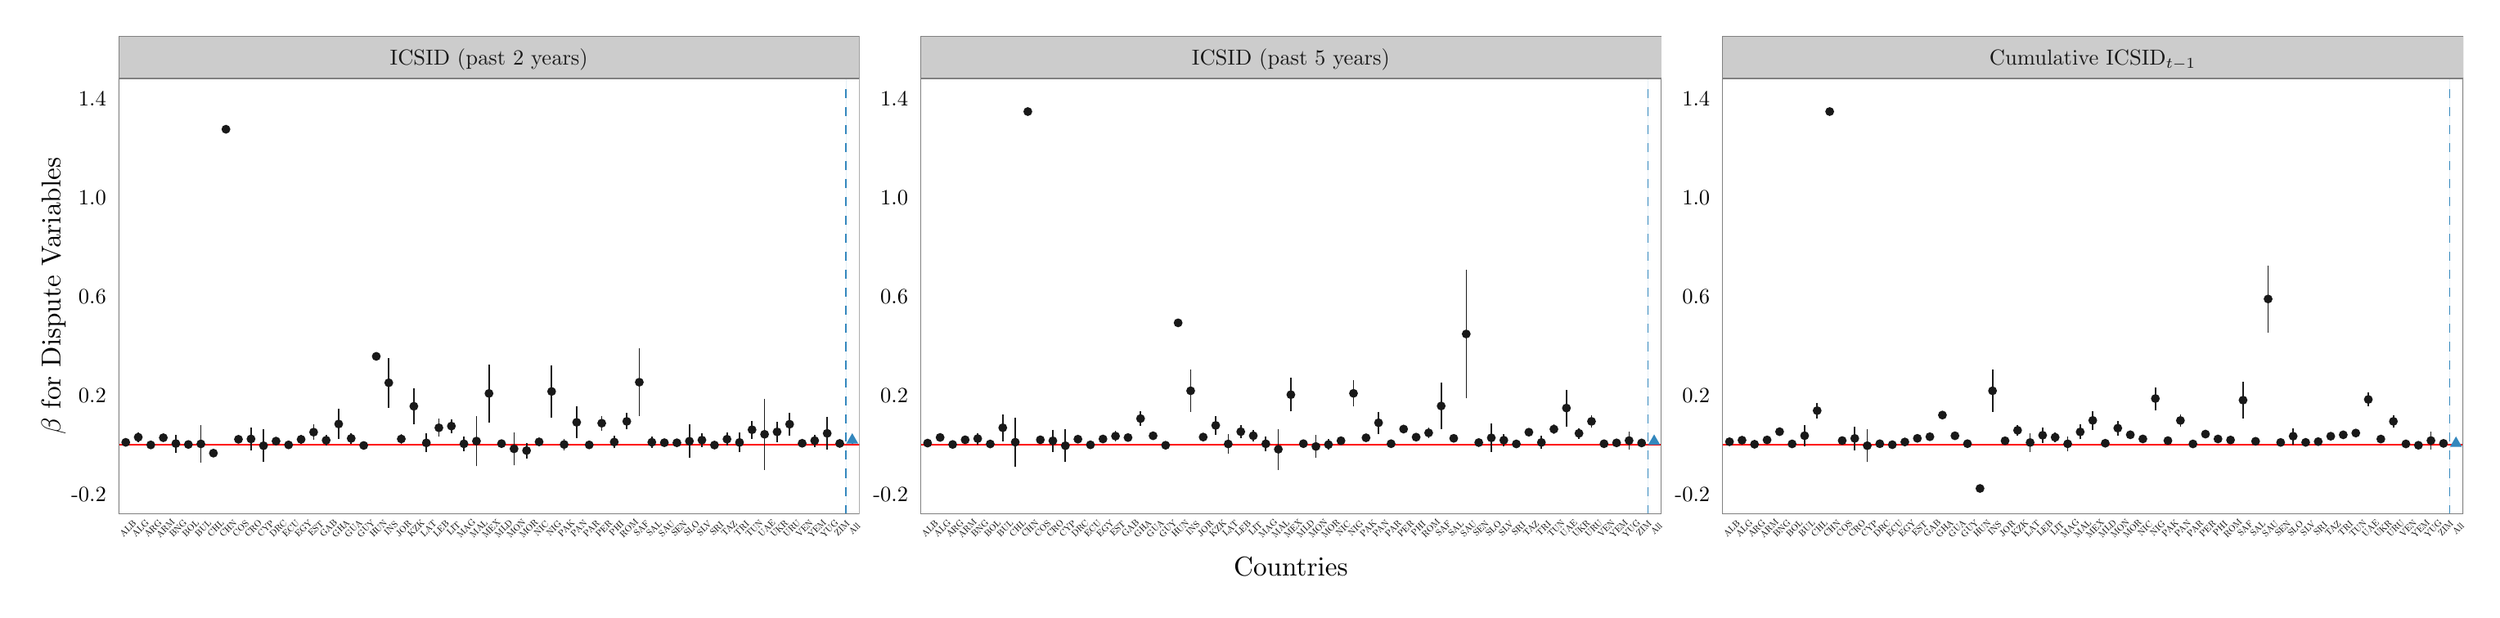
\begin{tikzpicture}[x=1pt,y=1pt]
\definecolor[named]{drawColor}{rgb}{0.00,0.00,0.00}
\definecolor[named]{fillColor}{rgb}{1.00,1.00,1.00}
\fill[color=fillColor,] (0,0) rectangle (1084.05,252.94);
\begin{scope}
\path[clip] (  0.00,  0.00) rectangle (1084.05,252.94);
\end{scope}
\begin{scope}
\path[clip] (  0.00,  0.00) rectangle (1084.05,252.94);
\end{scope}
\begin{scope}
\path[clip] (  0.00,  0.00) rectangle (1084.05,252.94);
\end{scope}
\begin{scope}
\path[clip] (  0.00,  0.00) rectangle (1084.05,252.94);
\end{scope}
\begin{scope}
\path[clip] (  0.00,  0.00) rectangle (1084.05,252.94);
\end{scope}
\begin{scope}
\path[clip] (  0.00,  0.00) rectangle (1084.05,252.94);
\end{scope}
\begin{scope}
\path[clip] (  0.00,  0.00) rectangle (1084.05,252.94);
\end{scope}
\begin{scope}
\path[clip] (  0.00,  0.00) rectangle (1084.05,252.94);
\end{scope}
\begin{scope}
\path[clip] (  0.00,  0.00) rectangle (1084.05,252.94);
\end{scope}
\begin{scope}
\path[clip] (  0.00,  0.00) rectangle (1084.05,252.94);
\end{scope}
\begin{scope}
\path[clip] (  0.00,  0.00) rectangle (1084.05,252.94);
\end{scope}
\begin{scope}
\path[clip] (  0.00,  0.00) rectangle (1084.05,252.94);
\end{scope}
\begin{scope}
\path[clip] (  0.00,  0.00) rectangle (1084.05,252.94);
\end{scope}
\begin{scope}
\path[clip] (  0.00,  0.00) rectangle (1084.05,252.94);
\end{scope}
\begin{scope}
\path[clip] (  0.00,  0.00) rectangle (1084.05,252.94);
\end{scope}
\begin{scope}
\path[clip] (  0.00,  0.00) rectangle (1084.05,252.94);
\definecolor[named]{drawColor}{rgb}{1.00,1.00,1.00}
\definecolor[named]{fillColor}{rgb}{1.00,1.00,1.00}

\draw[color=drawColor,line width= 0.6pt,line cap=round,line join=round,fill=fillColor,] (  0.00,  0.00) rectangle (1084.05,252.94);
\end{scope}
\begin{scope}
\path[clip] (  0.00,  0.00) rectangle (1084.05,252.94);
\end{scope}
\begin{scope}
\path[clip] ( 42.33, 35.72) rectangle (369.66,228.33);
\definecolor[named]{fillColor}{rgb}{1.00,1.00,1.00}

\draw[fill=fillColor,draw opacity=0.00,] ( 42.33, 35.72) rectangle (369.66,228.33);
\definecolor[named]{drawColor}{rgb}{1.00,0.00,0.00}
\definecolor[named]{fillColor}{rgb}{1.00,0.00,0.00}

\draw[color=drawColor,line width= 0.6pt,line join=round,fill=fillColor,] ( 42.33, 66.37) -- (369.66, 66.37);
\definecolor[named]{fillColor}{rgb}{0.10,0.10,0.10}

\draw[fill=fillColor,draw opacity=0.00,] (316.65, 67.36) circle (  1.96);

\draw[fill=fillColor,draw opacity=0.00,] (205.99, 89.03) circle (  1.96);

\draw[fill=fillColor,draw opacity=0.00,] (145.13, 69.14) circle (  1.96);

\draw[fill=fillColor,draw opacity=0.00,] (277.92, 67.45) circle (  1.96);

\draw[fill=fillColor,draw opacity=0.00,] (228.13, 67.61) circle (  1.96);

\draw[fill=fillColor,draw opacity=0.00,] ( 95.33, 68.75) circle (  1.96);

\draw[fill=fillColor,draw opacity=0.00,] (244.72, 76.26) circle (  1.96);

\draw[fill=fillColor,draw opacity=0.00,] (344.32, 67.00) circle (  1.96);

\draw[fill=fillColor,draw opacity=0.00,] (150.66, 66.03) circle (  1.96);

\draw[fill=fillColor,draw opacity=0.00,] (117.47, 66.28) circle (  1.96);

\draw[fill=fillColor,draw opacity=0.00,] (255.79, 75.87) circle (  1.96);

\draw[fill=fillColor,draw opacity=0.00,] ( 73.20, 66.46) circle (  1.96);

\draw[fill=fillColor,draw opacity=0.00,] (250.26, 66.28) circle (  1.96);

\draw[fill=fillColor,draw opacity=0.00,] ( 84.27, 62.63) circle (  1.96);

\draw[fill=fillColor,draw opacity=0.00,] ( 56.60, 66.27) circle (  1.96);

\draw[fill=fillColor,draw opacity=0.00,] (338.79, 75.42) circle (  1.96);

\draw[fill=fillColor,draw opacity=0.00,] (156.20,105.42) circle (  1.96);

\draw[fill=fillColor,draw opacity=0.00,] (294.52, 67.92) circle (  1.96);

\draw[fill=fillColor,draw opacity=0.00,] ( 45.54, 67.41) circle (  1.96);

\draw[fill=fillColor,draw opacity=0.00,] (100.87, 68.91) circle (  1.96);

\draw[fill=fillColor,draw opacity=0.00,] (355.38, 71.38) circle (  1.96);

\draw[fill=fillColor,draw opacity=0.00,] (300.05, 68.40) circle (  1.96);

\draw[fill=fillColor,draw opacity=0.00,] (106.40, 65.92) circle (  1.96);

\draw[fill=fillColor,draw opacity=0.00,] ( 78.73, 66.72) circle (  1.96);

\draw[fill=fillColor,draw opacity=0.00,] (211.53, 66.84) circle (  1.96);

\draw[fill=fillColor,draw opacity=0.00,] (266.86, 76.68) circle (  1.96);

\draw[fill=fillColor,draw opacity=0.00,] (128.53, 71.92) circle (  1.96);

\draw[fill=fillColor,draw opacity=0.00,] (178.33, 67.16) circle (  1.96);

\draw[fill=fillColor,draw opacity=0.00,] (189.39, 74.59) circle (  1.96);

\draw[fill=fillColor,draw opacity=0.00,] (333.25, 72.04) circle (  1.96);

\draw[fill=fillColor,draw opacity=0.00,] ( 62.14, 69.45) circle (  1.96);

\draw[fill=fillColor,draw opacity=0.00,] (288.99, 67.21) circle (  1.96);

\draw[fill=fillColor,draw opacity=0.00,] (139.60, 75.52) circle (  1.96);

\draw[fill=fillColor,draw opacity=0.00,] (233.66, 89.90) circle (  1.96);

\draw[fill=fillColor,draw opacity=0.00,] (134.06, 68.32) circle (  1.96);

\draw[fill=fillColor,draw opacity=0.00,] (111.93, 67.94) circle (  1.96);

\draw[fill=fillColor,draw opacity=0.00,] (311.12, 68.80) circle (  1.96);

\draw[fill=fillColor,draw opacity=0.00,] (360.92, 66.92) circle (  1.96);

\draw[fill=fillColor,draw opacity=0.00,] (272.39, 93.99) circle (  1.96);

\draw[fill=fillColor,draw opacity=0.00,] (194.93, 66.76) circle (  1.96);

\draw[fill=fillColor,draw opacity=0.00,] (222.59, 63.77) circle (  1.96);

\draw[fill=fillColor,draw opacity=0.00,] ( 51.07, 69.67) circle (  1.96);

\draw[fill=fillColor,draw opacity=0.00,] (322.19, 72.98) circle (  1.96);

\draw[fill=fillColor,draw opacity=0.00,] (123.00, 68.72) circle (  1.96);

\draw[fill=fillColor,draw opacity=0.00,] (183.86, 73.84) circle (  1.96);

\draw[fill=fillColor,draw opacity=0.00,] (167.26, 68.90) circle (  1.96);

\draw[fill=fillColor,draw opacity=0.00,] (283.46, 67.25) circle (  1.96);

\draw[fill=fillColor,draw opacity=0.00,] (349.85, 68.16) circle (  1.96);

\draw[fill=fillColor,draw opacity=0.00,] (327.72, 70.97) circle (  1.96);

\draw[fill=fillColor,draw opacity=0.00,] (172.80, 83.36) circle (  1.96);

\draw[fill=fillColor,draw opacity=0.00,] ( 89.80,205.80) circle (  1.96);

\draw[fill=fillColor,draw opacity=0.00,] (217.06, 64.55) circle (  1.96);

\draw[fill=fillColor,draw opacity=0.00,] (239.19, 66.47) circle (  1.96);

\draw[fill=fillColor,draw opacity=0.00,] ( 67.67, 66.87) circle (  1.96);

\draw[fill=fillColor,draw opacity=0.00,] (305.59, 66.20) circle (  1.96);

\draw[fill=fillColor,draw opacity=0.00,] (200.46, 67.96) circle (  1.96);

\draw[fill=fillColor,draw opacity=0.00,] (261.32, 67.54) circle (  1.96);

\draw[fill=fillColor,draw opacity=0.00,] (161.73, 93.74) circle (  1.96);
\definecolor[named]{fillColor}{rgb}{0.20,0.53,0.74}

\draw[fill=fillColor,draw opacity=0.00,] (366.45, 71.45) --
	(369.09, 66.87) --
	(363.81, 66.87) --
	cycle;
\definecolor[named]{drawColor}{rgb}{0.20,0.53,0.74}

\draw[color=drawColor,line width= 0.6pt,dash pattern=on 4pt off 4pt ,line join=round,fill=fillColor,] (363.68, 35.72) -- (363.68,228.33);
\definecolor[named]{drawColor}{rgb}{0.10,0.10,0.10}
\definecolor[named]{fillColor}{rgb}{0.10,0.10,0.10}

\draw[color=drawColor,line width= 0.6pt,line join=round,fill=fillColor,] (316.65, 63.09) -- (316.65, 71.64);

\draw[color=drawColor,line width= 0.6pt,line join=round,fill=fillColor,] (205.99, 76.16) -- (205.99,101.89);

\draw[color=drawColor,line width= 0.6pt,line join=round,fill=fillColor,] (145.13, 66.83) -- (145.13, 71.45);

\draw[color=drawColor,line width= 0.6pt,line join=round,fill=fillColor,] (277.92, 64.93) -- (277.92, 69.97);

\draw[color=drawColor,line width= 0.6pt,line join=round,fill=fillColor,] (228.13, 65.96) -- (228.13, 69.26);

\draw[color=drawColor,line width= 0.6pt,line join=round,fill=fillColor,] ( 95.33, 67.42) -- ( 95.33, 70.08);

\draw[color=drawColor,line width= 0.6pt,line join=round,fill=fillColor,] (244.72, 69.34) -- (244.72, 83.18);

\draw[color=drawColor,line width= 0.6pt,line join=round,fill=fillColor,] (344.32, 66.20) -- (344.32, 67.79);

\draw[color=drawColor,line width= 0.6pt,line join=round,fill=fillColor,] (150.66, 65.53) -- (150.66, 66.54);

\draw[color=drawColor,line width= 0.6pt,line join=round,fill=fillColor,] (117.47, 65.88) -- (117.47, 66.69);

\draw[color=drawColor,line width= 0.6pt,line join=round,fill=fillColor,] (255.79, 72.56) -- (255.79, 79.18);

\draw[color=drawColor,line width= 0.6pt,line join=round,fill=fillColor,] ( 73.20, 65.41) -- ( 73.20, 67.51);

\draw[color=drawColor,line width= 0.6pt,line join=round,fill=fillColor,] (250.26, 65.78) -- (250.26, 66.79);

\draw[color=drawColor,line width= 0.6pt,line join=round,fill=fillColor,] ( 56.60, 65.24) -- ( 56.60, 67.29);

\draw[color=drawColor,line width= 0.6pt,line join=round,fill=fillColor,] (338.79, 70.25) -- (338.79, 80.59);

\draw[color=drawColor,line width= 0.6pt,line join=round,fill=fillColor,] (294.52, 60.56) -- (294.52, 75.28);

\draw[color=drawColor,line width= 0.6pt,line join=round,fill=fillColor,] ( 45.54, 66.30) -- ( 45.54, 68.52);

\draw[color=drawColor,line width= 0.6pt,line join=round,fill=fillColor,] (100.87, 63.80) -- (100.87, 74.02);

\draw[color=drawColor,line width= 0.6pt,line join=round,fill=fillColor,] (355.38, 64.18) -- (355.38, 78.57);

\draw[color=drawColor,line width= 0.6pt,line join=round,fill=fillColor,] (300.05, 65.33) -- (300.05, 71.48);

\draw[color=drawColor,line width= 0.6pt,line join=round,fill=fillColor,] (106.40, 58.62) -- (106.40, 73.22);

\draw[color=drawColor,line width= 0.6pt,line join=round,fill=fillColor,] ( 78.73, 58.51) -- ( 78.73, 74.92);

\draw[color=drawColor,line width= 0.6pt,line join=round,fill=fillColor,] (211.53, 65.68) -- (211.53, 68.00);

\draw[color=drawColor,line width= 0.6pt,line join=round,fill=fillColor,] (266.86, 73.07) -- (266.86, 80.29);

\draw[color=drawColor,line width= 0.6pt,line join=round,fill=fillColor,] (128.53, 68.47) -- (128.53, 75.38);

\draw[color=drawColor,line width= 0.6pt,line join=round,fill=fillColor,] (178.33, 63.07) -- (178.33, 71.25);

\draw[color=drawColor,line width= 0.6pt,line join=round,fill=fillColor,] (189.39, 71.54) -- (189.39, 77.64);

\draw[color=drawColor,line width= 0.6pt,line join=round,fill=fillColor,] (333.25, 67.55) -- (333.25, 76.53);

\draw[color=drawColor,line width= 0.6pt,line join=round,fill=fillColor,] ( 62.14, 68.10) -- ( 62.14, 70.79);

\draw[color=drawColor,line width= 0.6pt,line join=round,fill=fillColor,] (288.99, 66.37) -- (288.99, 68.05);

\draw[color=drawColor,line width= 0.6pt,line join=round,fill=fillColor,] (139.60, 68.86) -- (139.60, 82.17);

\draw[color=drawColor,line width= 0.6pt,line join=round,fill=fillColor,] (233.66, 78.22) -- (233.66,101.57);

\draw[color=drawColor,line width= 0.6pt,line join=round,fill=fillColor,] (134.06, 65.86) -- (134.06, 70.78);

\draw[color=drawColor,line width= 0.6pt,line join=round,fill=fillColor,] (111.93, 66.28) -- (111.93, 69.60);

\draw[color=drawColor,line width= 0.6pt,line join=round,fill=fillColor,] (311.12, 65.98) -- (311.12, 71.62);

\draw[color=drawColor,line width= 0.6pt,line join=round,fill=fillColor,] (360.92, 66.47) -- (360.92, 67.38);

\draw[color=drawColor,line width= 0.6pt,line join=round,fill=fillColor,] (272.39, 79.14) -- (272.39,108.85);

\draw[color=drawColor,line width= 0.6pt,line join=round,fill=fillColor,] (194.93, 63.42) -- (194.93, 70.09);

\draw[color=drawColor,line width= 0.6pt,line join=round,fill=fillColor,] (222.59, 60.34) -- (222.59, 67.20);

\draw[color=drawColor,line width= 0.6pt,line join=round,fill=fillColor,] ( 51.07, 67.55) -- ( 51.07, 71.79);

\draw[color=drawColor,line width= 0.6pt,line join=round,fill=fillColor,] (322.19, 68.94) -- (322.19, 77.02);

\draw[color=drawColor,line width= 0.6pt,line join=round,fill=fillColor,] (123.00, 66.61) -- (123.00, 70.83);

\draw[color=drawColor,line width= 0.6pt,line join=round,fill=fillColor,] (183.86, 69.87) -- (183.86, 77.80);

\draw[color=drawColor,line width= 0.6pt,line join=round,fill=fillColor,] (167.26, 66.77) -- (167.26, 71.04);

\draw[color=drawColor,line width= 0.6pt,line join=round,fill=fillColor,] (349.85, 65.45) -- (349.85, 70.87);

\draw[color=drawColor,line width= 0.6pt,line join=round,fill=fillColor,] (327.72, 55.33) -- (327.72, 86.61);

\draw[color=drawColor,line width= 0.6pt,line join=round,fill=fillColor,] (172.80, 75.54) -- (172.80, 91.18);

\draw[color=drawColor,line width= 0.6pt,line join=round,fill=fillColor,] (217.06, 57.15) -- (217.06, 71.96);

\draw[color=drawColor,line width= 0.6pt,line join=round,fill=fillColor,] (239.19, 63.94) -- (239.19, 69.00);

\draw[color=drawColor,line width= 0.6pt,line join=round,fill=fillColor,] ( 67.67, 62.92) -- ( 67.67, 70.83);

\draw[color=drawColor,line width= 0.6pt,line join=round,fill=fillColor,] (305.59, 65.07) -- (305.59, 67.32);

\draw[color=drawColor,line width= 0.6pt,line join=round,fill=fillColor,] (200.46, 56.82) -- (200.46, 79.10);

\draw[color=drawColor,line width= 0.6pt,line join=round,fill=fillColor,] (261.32, 64.80) -- (261.32, 70.28);

\draw[color=drawColor,line width= 0.6pt,line join=round,fill=fillColor,] (161.73, 82.73) -- (161.73,104.74);
\definecolor[named]{drawColor}{rgb}{0.20,0.53,0.74}
\definecolor[named]{fillColor}{rgb}{0.20,0.53,0.74}

\draw[color=drawColor,line width= 0.6pt,line join=round,fill=fillColor,] (366.45, 66.58) -- (366.45, 70.22);
\definecolor[named]{drawColor}{rgb}{0.50,0.50,0.50}

\draw[color=drawColor,line width= 0.6pt,line cap=round,line join=round,fill opacity=0.00,] ( 42.33, 35.72) rectangle (369.66,228.33);
\end{scope}
\begin{scope}
\path[clip] (  0.00,  0.00) rectangle (1084.05,252.94);
\end{scope}
\begin{scope}
\path[clip] (396.52, 35.72) rectangle (723.85,228.33);
\definecolor[named]{fillColor}{rgb}{1.00,1.00,1.00}

\draw[fill=fillColor,draw opacity=0.00,] (396.52, 35.72) rectangle (723.85,228.33);
\definecolor[named]{drawColor}{rgb}{1.00,0.00,0.00}
\definecolor[named]{fillColor}{rgb}{1.00,0.00,0.00}

\draw[color=drawColor,line width= 0.6pt,line join=round,fill=fillColor,] (396.52, 66.37) -- (723.85, 66.37);
\definecolor[named]{fillColor}{rgb}{0.10,0.10,0.10}

\draw[fill=fillColor,draw opacity=0.00,] (670.85, 67.36) circle (  1.96);

\draw[fill=fillColor,draw opacity=0.00,] (560.19, 88.48) circle (  1.96);

\draw[fill=fillColor,draw opacity=0.00,] (499.33, 70.31) circle (  1.96);

\draw[fill=fillColor,draw opacity=0.00,] (632.12, 69.18) circle (  1.96);

\draw[fill=fillColor,draw opacity=0.00,] (582.32, 68.12) circle (  1.96);

\draw[fill=fillColor,draw opacity=0.00,] (449.53, 68.53) circle (  1.96);

\draw[fill=fillColor,draw opacity=0.00,] (598.92, 76.06) circle (  1.96);

\draw[fill=fillColor,draw opacity=0.00,] (698.51, 66.79) circle (  1.96);

\draw[fill=fillColor,draw opacity=0.00,] (504.86, 66.12) circle (  1.96);

\draw[fill=fillColor,draw opacity=0.00,] (471.66, 66.31) circle (  1.96);

\draw[fill=fillColor,draw opacity=0.00,] (609.99, 73.27) circle (  1.96);

\draw[fill=fillColor,draw opacity=0.00,] (427.40, 66.69) circle (  1.96);

\draw[fill=fillColor,draw opacity=0.00,] (604.45, 66.80) circle (  1.96);

\draw[fill=fillColor,draw opacity=0.00,] (438.46, 67.48) circle (  1.96);

\draw[fill=fillColor,draw opacity=0.00,] (410.80, 66.47) circle (  1.96);

\draw[fill=fillColor,draw opacity=0.00,] (692.98, 76.68) circle (  1.96);

\draw[fill=fillColor,draw opacity=0.00,] (510.39,120.23) circle (  1.96);

\draw[fill=fillColor,draw opacity=0.00,] (648.72, 69.41) circle (  1.96);

\draw[fill=fillColor,draw opacity=0.00,] (399.73, 67.07) circle (  1.96);

\draw[fill=fillColor,draw opacity=0.00,] (455.06, 68.08) circle (  1.96);

\draw[fill=fillColor,draw opacity=0.00,] (709.58, 68.20) circle (  1.96);

\draw[fill=fillColor,draw opacity=0.00,] (654.25, 68.35) circle (  1.96);

\draw[fill=fillColor,draw opacity=0.00,] (460.59, 65.92) circle (  1.96);

\draw[fill=fillColor,draw opacity=0.00,] (432.93, 73.86) circle (  1.96);

\draw[fill=fillColor,draw opacity=0.00,] (565.72, 66.82) circle (  1.96);

\draw[fill=fillColor,draw opacity=0.00,] (621.05, 71.60) circle (  1.96);

\draw[fill=fillColor,draw opacity=0.00,] (482.73, 70.16) circle (  1.96);

\draw[fill=fillColor,draw opacity=0.00,] (532.52, 66.69) circle (  1.96);

\draw[fill=fillColor,draw opacity=0.00,] (543.59, 70.33) circle (  1.96);

\draw[fill=fillColor,draw opacity=0.00,] (687.45, 71.38) circle (  1.96);

\draw[fill=fillColor,draw opacity=0.00,] (416.33, 68.53) circle (  1.96);

\draw[fill=fillColor,draw opacity=0.00,] (643.18, 67.31) circle (  1.96);

\draw[fill=fillColor,draw opacity=0.00,] (493.79, 77.91) circle (  1.96);

\draw[fill=fillColor,draw opacity=0.00,] (587.85, 89.07) circle (  1.96);

\draw[fill=fillColor,draw opacity=0.00,] (488.26, 69.52) circle (  1.96);

\draw[fill=fillColor,draw opacity=0.00,] (466.13, 68.81) circle (  1.96);

\draw[fill=fillColor,draw opacity=0.00,] (665.32, 71.89) circle (  1.96);

\draw[fill=fillColor,draw opacity=0.00,] (715.11, 67.13) circle (  1.96);

\draw[fill=fillColor,draw opacity=0.00,] (626.58, 83.48) circle (  1.96);

\draw[fill=fillColor,draw opacity=0.00,] (549.12, 66.76) circle (  1.96);

\draw[fill=fillColor,draw opacity=0.00,] (576.79, 66.43) circle (  1.96);

\draw[fill=fillColor,draw opacity=0.00,] (405.26, 69.57) circle (  1.96);

\draw[fill=fillColor,draw opacity=0.00,] (676.38, 73.24) circle (  1.96);

\draw[fill=fillColor,draw opacity=0.00,] (477.19, 68.89) circle (  1.96);

\draw[fill=fillColor,draw opacity=0.00,] (538.06, 72.12) circle (  1.96);

\draw[fill=fillColor,draw opacity=0.00,] (521.46, 69.74) circle (  1.96);

\draw[fill=fillColor,draw opacity=0.00,] (637.65,115.31) circle (  1.96);

\draw[fill=fillColor,draw opacity=0.00,] (704.05, 67.17) circle (  1.96);

\draw[fill=fillColor,draw opacity=0.00,] (681.91, 82.57) circle (  1.96);

\draw[fill=fillColor,draw opacity=0.00,] (526.99, 74.90) circle (  1.96);

\draw[fill=fillColor,draw opacity=0.00,] (444.00,213.62) circle (  1.96);

\draw[fill=fillColor,draw opacity=0.00,] (571.25, 65.59) circle (  1.96);

\draw[fill=fillColor,draw opacity=0.00,] (593.39, 69.42) circle (  1.96);

\draw[fill=fillColor,draw opacity=0.00,] (421.86, 69.06) circle (  1.96);

\draw[fill=fillColor,draw opacity=0.00,] (659.78, 66.71) circle (  1.96);

\draw[fill=fillColor,draw opacity=0.00,] (554.66, 64.35) circle (  1.96);

\draw[fill=fillColor,draw opacity=0.00,] (615.52, 69.70) circle (  1.96);

\draw[fill=fillColor,draw opacity=0.00,] (515.92, 90.19) circle (  1.96);
\definecolor[named]{fillColor}{rgb}{0.20,0.53,0.74}

\draw[fill=fillColor,draw opacity=0.00,] (720.65, 70.91) --
	(723.29, 66.33) --
	(718.00, 66.33) --
	cycle;
\definecolor[named]{drawColor}{rgb}{0.20,0.53,0.74}

\draw[color=drawColor,line width= 0.6pt,dash pattern=on 4pt off 4pt ,line join=round,fill=fillColor,] (717.88, 35.72) -- (717.88,228.33);
\definecolor[named]{drawColor}{rgb}{0.10,0.10,0.10}
\definecolor[named]{fillColor}{rgb}{0.10,0.10,0.10}

\draw[color=drawColor,line width= 0.6pt,line join=round,fill=fillColor,] (670.85, 64.51) -- (670.85, 70.22);

\draw[color=drawColor,line width= 0.6pt,line join=round,fill=fillColor,] (560.19, 81.07) -- (560.19, 95.90);

\draw[color=drawColor,line width= 0.6pt,line join=round,fill=fillColor,] (499.33, 69.22) -- (499.33, 71.40);

\draw[color=drawColor,line width= 0.6pt,line join=round,fill=fillColor,] (632.12, 67.73) -- (632.12, 70.64);

\draw[color=drawColor,line width= 0.6pt,line join=round,fill=fillColor,] (582.32, 67.13) -- (582.32, 69.12);

\draw[color=drawColor,line width= 0.6pt,line join=round,fill=fillColor,] (449.53, 68.00) -- (449.53, 69.06);

\draw[color=drawColor,line width= 0.6pt,line join=round,fill=fillColor,] (598.92, 71.24) -- (598.92, 80.87);

\draw[color=drawColor,line width= 0.6pt,line join=round,fill=fillColor,] (698.51, 66.22) -- (698.51, 67.35);

\draw[color=drawColor,line width= 0.6pt,line join=round,fill=fillColor,] (504.86, 65.79) -- (504.86, 66.46);

\draw[color=drawColor,line width= 0.6pt,line join=round,fill=fillColor,] (471.66, 66.12) -- (471.66, 66.49);

\draw[color=drawColor,line width= 0.6pt,line join=round,fill=fillColor,] (609.99, 71.41) -- (609.99, 75.13);

\draw[color=drawColor,line width= 0.6pt,line join=round,fill=fillColor,] (427.40, 66.08) -- (427.40, 67.29);

\draw[color=drawColor,line width= 0.6pt,line join=round,fill=fillColor,] (604.45, 66.47) -- (604.45, 67.14);

\draw[color=drawColor,line width= 0.6pt,line join=round,fill=fillColor,] (438.46, 56.64) -- (438.46, 78.33);

\draw[color=drawColor,line width= 0.6pt,line join=round,fill=fillColor,] (410.80, 65.95) -- (410.80, 67.00);

\draw[color=drawColor,line width= 0.6pt,line join=round,fill=fillColor,] (692.98, 73.82) -- (692.98, 79.55);

\draw[color=drawColor,line width= 0.6pt,line join=round,fill=fillColor,] (648.72, 63.16) -- (648.72, 75.67);

\draw[color=drawColor,line width= 0.6pt,line join=round,fill=fillColor,] (399.73, 66.21) -- (399.73, 67.94);

\draw[color=drawColor,line width= 0.6pt,line join=round,fill=fillColor,] (455.06, 63.19) -- (455.06, 72.98);

\draw[color=drawColor,line width= 0.6pt,line join=round,fill=fillColor,] (709.58, 64.23) -- (709.58, 72.17);

\draw[color=drawColor,line width= 0.6pt,line join=round,fill=fillColor,] (654.25, 65.81) -- (654.25, 70.89);

\draw[color=drawColor,line width= 0.6pt,line join=round,fill=fillColor,] (460.59, 58.62) -- (460.59, 73.22);

\draw[color=drawColor,line width= 0.6pt,line join=round,fill=fillColor,] (432.93, 67.83) -- (432.93, 79.89);

\draw[color=drawColor,line width= 0.6pt,line join=round,fill=fillColor,] (565.72, 65.84) -- (565.72, 67.80);

\draw[color=drawColor,line width= 0.6pt,line join=round,fill=fillColor,] (621.05, 69.40) -- (621.05, 73.81);

\draw[color=drawColor,line width= 0.6pt,line join=round,fill=fillColor,] (482.73, 67.84) -- (482.73, 72.48);

\draw[color=drawColor,line width= 0.6pt,line join=round,fill=fillColor,] (532.52, 62.49) -- (532.52, 70.90);

\draw[color=drawColor,line width= 0.6pt,line join=round,fill=fillColor,] (543.59, 67.83) -- (543.59, 72.83);

\draw[color=drawColor,line width= 0.6pt,line join=round,fill=fillColor,] (687.45, 69.04) -- (687.45, 73.73);

\draw[color=drawColor,line width= 0.6pt,line join=round,fill=fillColor,] (416.33, 67.70) -- (416.33, 69.36);

\draw[color=drawColor,line width= 0.6pt,line join=round,fill=fillColor,] (643.18, 66.80) -- (643.18, 67.82);

\draw[color=drawColor,line width= 0.6pt,line join=round,fill=fillColor,] (493.79, 74.70) -- (493.79, 81.12);

\draw[color=drawColor,line width= 0.6pt,line join=round,fill=fillColor,] (587.85, 83.18) -- (587.85, 94.96);

\draw[color=drawColor,line width= 0.6pt,line join=round,fill=fillColor,] (488.26, 68.15) -- (488.26, 70.90);

\draw[color=drawColor,line width= 0.6pt,line join=round,fill=fillColor,] (466.13, 68.02) -- (466.13, 69.61);

\draw[color=drawColor,line width= 0.6pt,line join=round,fill=fillColor,] (665.32, 70.59) -- (665.32, 73.19);

\draw[color=drawColor,line width= 0.6pt,line join=round,fill=fillColor,] (715.11, 66.85) -- (715.11, 67.41);

\draw[color=drawColor,line width= 0.6pt,line join=round,fill=fillColor,] (626.58, 73.27) -- (626.58, 93.70);

\draw[color=drawColor,line width= 0.6pt,line join=round,fill=fillColor,] (549.12, 63.42) -- (549.12, 70.09);

\draw[color=drawColor,line width= 0.6pt,line join=round,fill=fillColor,] (576.79, 64.06) -- (576.79, 68.79);

\draw[color=drawColor,line width= 0.6pt,line join=round,fill=fillColor,] (405.26, 68.49) -- (405.26, 70.64);

\draw[color=drawColor,line width= 0.6pt,line join=round,fill=fillColor,] (676.38, 71.10) -- (676.38, 75.38);

\draw[color=drawColor,line width= 0.6pt,line join=round,fill=fillColor,] (477.19, 67.74) -- (477.19, 70.05);

\draw[color=drawColor,line width= 0.6pt,line join=round,fill=fillColor,] (538.06, 69.27) -- (538.06, 74.96);

\draw[color=drawColor,line width= 0.6pt,line join=round,fill=fillColor,] (521.46, 68.75) -- (521.46, 70.72);

\draw[color=drawColor,line width= 0.6pt,line join=round,fill=fillColor,] (637.65, 86.86) -- (637.65,143.77);

\draw[color=drawColor,line width= 0.6pt,line join=round,fill=fillColor,] (704.05, 65.39) -- (704.05, 68.95);

\draw[color=drawColor,line width= 0.6pt,line join=round,fill=fillColor,] (681.91, 74.44) -- (681.91, 90.70);

\draw[color=drawColor,line width= 0.6pt,line join=round,fill=fillColor,] (526.99, 70.69) -- (526.99, 79.10);

\draw[color=drawColor,line width= 0.6pt,line join=round,fill=fillColor,] (571.25, 60.56) -- (571.25, 70.62);

\draw[color=drawColor,line width= 0.6pt,line join=round,fill=fillColor,] (593.39, 68.21) -- (593.39, 70.63);

\draw[color=drawColor,line width= 0.6pt,line join=round,fill=fillColor,] (421.86, 66.54) -- (421.86, 71.57);

\draw[color=drawColor,line width= 0.6pt,line join=round,fill=fillColor,] (659.78, 65.80) -- (659.78, 67.61);

\draw[color=drawColor,line width= 0.6pt,line join=round,fill=fillColor,] (554.66, 55.33) -- (554.66, 73.37);

\draw[color=drawColor,line width= 0.6pt,line join=round,fill=fillColor,] (615.52, 67.93) -- (615.52, 71.48);

\draw[color=drawColor,line width= 0.6pt,line join=round,fill=fillColor,] (515.92, 80.82) -- (515.92, 99.55);
\definecolor[named]{drawColor}{rgb}{0.20,0.53,0.74}
\definecolor[named]{fillColor}{rgb}{0.20,0.53,0.74}

\draw[color=drawColor,line width= 0.6pt,line join=round,fill=fillColor,] (720.65, 66.81) -- (720.65, 68.91);
\definecolor[named]{drawColor}{rgb}{0.50,0.50,0.50}

\draw[color=drawColor,line width= 0.6pt,line cap=round,line join=round,fill opacity=0.00,] (396.52, 35.72) rectangle (723.85,228.33);
\end{scope}
\begin{scope}
\path[clip] (  0.00,  0.00) rectangle (1084.05,252.94);
\end{scope}
\begin{scope}
\path[clip] (750.72, 35.72) rectangle (1078.05,228.33);
\definecolor[named]{fillColor}{rgb}{1.00,1.00,1.00}

\draw[fill=fillColor,draw opacity=0.00,] (750.72, 35.72) rectangle (1078.05,228.33);
\definecolor[named]{drawColor}{rgb}{1.00,0.00,0.00}
\definecolor[named]{fillColor}{rgb}{1.00,0.00,0.00}

\draw[color=drawColor,line width= 0.6pt,line join=round,fill=fillColor,] (750.72, 66.37) -- (1078.05, 66.37);
\definecolor[named]{fillColor}{rgb}{0.10,0.10,0.10}

\draw[fill=fillColor,draw opacity=0.00,] (1025.04, 70.73) circle (  1.96);

\draw[fill=fillColor,draw opacity=0.00,] (914.38, 77.11) circle (  1.96);

\draw[fill=fillColor,draw opacity=0.00,] (853.52, 70.31) circle (  1.96);

\draw[fill=fillColor,draw opacity=0.00,] (986.31, 67.87) circle (  1.96);

\draw[fill=fillColor,draw opacity=0.00,] (936.52, 68.91) circle (  1.96);

\draw[fill=fillColor,draw opacity=0.00,] (803.72, 68.19) circle (  1.96);

\draw[fill=fillColor,draw opacity=0.00,] (953.11, 77.07) circle (  1.96);

\draw[fill=fillColor,draw opacity=0.00,] (1052.71, 66.71) circle (  1.96);

\draw[fill=fillColor,draw opacity=0.00,] (859.05, 66.82) circle (  1.96);

\draw[fill=fillColor,draw opacity=0.00,] (825.86, 66.37) circle (  1.96);

\draw[fill=fillColor,draw opacity=0.00,] (964.18, 71.05) circle (  1.96);

\draw[fill=fillColor,draw opacity=0.00,] (781.59, 66.72) circle (  1.96);

\draw[fill=fillColor,draw opacity=0.00,] (958.65, 66.71) circle (  1.96);

\draw[fill=fillColor,draw opacity=0.00,] (792.66, 81.42) circle (  1.96);

\draw[fill=fillColor,draw opacity=0.00,] (764.99, 66.56) circle (  1.96);

\draw[fill=fillColor,draw opacity=0.00,] (1047.18, 76.68) circle (  1.96);

\draw[fill=fillColor,draw opacity=0.00,] (864.59, 47.02) circle (  1.96);

\draw[fill=fillColor,draw opacity=0.00,] (1002.91, 70.13) circle (  1.96);

\draw[fill=fillColor,draw opacity=0.00,] (753.93, 67.67) circle (  1.96);

\draw[fill=fillColor,draw opacity=0.00,] (809.26, 69.15) circle (  1.96);

\draw[fill=fillColor,draw opacity=0.00,] (1063.77, 68.20) circle (  1.96);

\draw[fill=fillColor,draw opacity=0.00,] (1008.44, 67.40) circle (  1.96);

\draw[fill=fillColor,draw opacity=0.00,] (814.79, 65.92) circle (  1.96);

\draw[fill=fillColor,draw opacity=0.00,] (787.12, 70.34) circle (  1.96);

\draw[fill=fillColor,draw opacity=0.00,] (919.92, 67.01) circle (  1.96);

\draw[fill=fillColor,draw opacity=0.00,] (975.25, 68.44) circle (  1.96);

\draw[fill=fillColor,draw opacity=0.00,] (836.92, 69.18) circle (  1.96);

\draw[fill=fillColor,draw opacity=0.00,] (886.72, 67.33) circle (  1.96);

\draw[fill=fillColor,draw opacity=0.00,] (897.78, 69.64) circle (  1.96);

\draw[fill=fillColor,draw opacity=0.00,] (1041.64, 68.86) circle (  1.96);

\draw[fill=fillColor,draw opacity=0.00,] (770.53, 68.47) circle (  1.96);

\draw[fill=fillColor,draw opacity=0.00,] (997.38, 67.37) circle (  1.96);

\draw[fill=fillColor,draw opacity=0.00,] (847.99, 79.47) circle (  1.96);

\draw[fill=fillColor,draw opacity=0.00,] (942.05, 86.77) circle (  1.96);

\draw[fill=fillColor,draw opacity=0.00,] (842.45, 69.89) circle (  1.96);

\draw[fill=fillColor,draw opacity=0.00,] (820.32, 66.79) circle (  1.96);

\draw[fill=fillColor,draw opacity=0.00,] (1019.51, 70.11) circle (  1.96);

\draw[fill=fillColor,draw opacity=0.00,] (1069.31, 66.94) circle (  1.96);

\draw[fill=fillColor,draw opacity=0.00,] (980.78, 86.06) circle (  1.96);

\draw[fill=fillColor,draw opacity=0.00,] (903.32, 66.76) circle (  1.96);

\draw[fill=fillColor,draw opacity=0.00,] (930.98, 70.75) circle (  1.96);

\draw[fill=fillColor,draw opacity=0.00,] (759.46, 68.35) circle (  1.96);

\draw[fill=fillColor,draw opacity=0.00,] (1030.58, 71.52) circle (  1.96);

\draw[fill=fillColor,draw opacity=0.00,] (831.39, 67.57) circle (  1.96);

\draw[fill=fillColor,draw opacity=0.00,] (892.25, 70.54) circle (  1.96);

\draw[fill=fillColor,draw opacity=0.00,] (875.65, 68.09) circle (  1.96);

\draw[fill=fillColor,draw opacity=0.00,] (991.85,130.78) circle (  1.96);

\draw[fill=fillColor,draw opacity=0.00,] (1058.24, 66.12) circle (  1.96);

\draw[fill=fillColor,draw opacity=0.00,] (1036.11, 86.36) circle (  1.96);

\draw[fill=fillColor,draw opacity=0.00,] (881.19, 72.73) circle (  1.96);

\draw[fill=fillColor,draw opacity=0.00,] (798.19,213.62) circle (  1.96);

\draw[fill=fillColor,draw opacity=0.00,] (925.45, 73.68) circle (  1.96);

\draw[fill=fillColor,draw opacity=0.00,] (947.58, 68.16) circle (  1.96);

\draw[fill=fillColor,draw opacity=0.00,] (776.06, 72.11) circle (  1.96);

\draw[fill=fillColor,draw opacity=0.00,] (1013.98, 67.73) circle (  1.96);

\draw[fill=fillColor,draw opacity=0.00,] (908.85, 72.02) circle (  1.96);

\draw[fill=fillColor,draw opacity=0.00,] (969.71, 68.90) circle (  1.96);

\draw[fill=fillColor,draw opacity=0.00,] (870.12, 90.19) circle (  1.96);
\definecolor[named]{fillColor}{rgb}{0.20,0.53,0.74}

\draw[fill=fillColor,draw opacity=0.00,] (1074.84, 70.01) --
	(1077.48, 65.43) --
	(1072.20, 65.43) --
	cycle;
\definecolor[named]{drawColor}{rgb}{0.20,0.53,0.74}

\draw[color=drawColor,line width= 0.6pt,dash pattern=on 4pt off 4pt ,line join=round,fill=fillColor,] (1072.07, 35.72) -- (1072.07,228.33);
\definecolor[named]{drawColor}{rgb}{0.10,0.10,0.10}
\definecolor[named]{fillColor}{rgb}{0.10,0.10,0.10}

\draw[color=drawColor,line width= 0.6pt,line join=round,fill=fillColor,] (1025.04, 69.03) -- (1025.04, 72.42);

\draw[color=drawColor,line width= 0.6pt,line join=round,fill=fillColor,] (914.38, 72.98) -- (914.38, 81.24);

\draw[color=drawColor,line width= 0.6pt,line join=round,fill=fillColor,] (853.52, 69.22) -- (853.52, 71.40);

\draw[color=drawColor,line width= 0.6pt,line join=round,fill=fillColor,] (986.31, 66.63) -- (986.31, 69.11);

\draw[color=drawColor,line width= 0.6pt,line join=round,fill=fillColor,] (936.52, 68.37) -- (936.52, 69.44);

\draw[color=drawColor,line width= 0.6pt,line join=round,fill=fillColor,] (803.72, 67.76) -- (803.72, 68.62);

\draw[color=drawColor,line width= 0.6pt,line join=round,fill=fillColor,] (953.11, 74.35) -- (953.11, 79.80);

\draw[color=drawColor,line width= 0.6pt,line join=round,fill=fillColor,] (1052.71, 66.26) -- (1052.71, 67.16);

\draw[color=drawColor,line width= 0.6pt,line join=round,fill=fillColor,] (859.05, 66.60) -- (859.05, 67.04);

\draw[color=drawColor,line width= 0.6pt,line join=round,fill=fillColor,] (825.86, 66.25) -- (825.86, 66.48);

\draw[color=drawColor,line width= 0.6pt,line join=round,fill=fillColor,] (964.18, 69.99) -- (964.18, 72.11);

\draw[color=drawColor,line width= 0.6pt,line join=round,fill=fillColor,] (781.59, 66.34) -- (781.59, 67.09);

\draw[color=drawColor,line width= 0.6pt,line join=round,fill=fillColor,] (958.65, 66.51) -- (958.65, 66.92);

\draw[color=drawColor,line width= 0.6pt,line join=round,fill=fillColor,] (792.66, 78.03) -- (792.66, 84.80);

\draw[color=drawColor,line width= 0.6pt,line join=round,fill=fillColor,] (764.99, 66.27) -- (764.99, 66.86);

\draw[color=drawColor,line width= 0.6pt,line join=round,fill=fillColor,] (1047.18, 73.82) -- (1047.18, 79.55);

\draw[color=drawColor,line width= 0.6pt,line join=round,fill=fillColor,] (1002.91, 66.49) -- (1002.91, 73.77);

\draw[color=drawColor,line width= 0.6pt,line join=round,fill=fillColor,] (753.93, 67.27) -- (753.93, 68.07);

\draw[color=drawColor,line width= 0.6pt,line join=round,fill=fillColor,] (809.26, 64.00) -- (809.26, 74.30);

\draw[color=drawColor,line width= 0.6pt,line join=round,fill=fillColor,] (1063.77, 64.23) -- (1063.77, 72.17);

\draw[color=drawColor,line width= 0.6pt,line join=round,fill=fillColor,] (1008.44, 65.61) -- (1008.44, 69.19);

\draw[color=drawColor,line width= 0.6pt,line join=round,fill=fillColor,] (814.79, 58.62) -- (814.79, 73.22);

\draw[color=drawColor,line width= 0.6pt,line join=round,fill=fillColor,] (787.12, 65.65) -- (787.12, 75.04);

\draw[color=drawColor,line width= 0.6pt,line join=round,fill=fillColor,] (919.92, 66.07) -- (919.92, 67.95);

\draw[color=drawColor,line width= 0.6pt,line join=round,fill=fillColor,] (975.25, 66.94) -- (975.25, 69.93);

\draw[color=drawColor,line width= 0.6pt,line join=round,fill=fillColor,] (836.92, 68.26) -- (836.92, 70.11);

\draw[color=drawColor,line width= 0.6pt,line join=round,fill=fillColor,] (886.72, 63.25) -- (886.72, 71.41);

\draw[color=drawColor,line width= 0.6pt,line join=round,fill=fillColor,] (897.78, 67.44) -- (897.78, 71.84);

\draw[color=drawColor,line width= 0.6pt,line join=round,fill=fillColor,] (1041.64, 67.80) -- (1041.64, 69.92);

\draw[color=drawColor,line width= 0.6pt,line join=round,fill=fillColor,] (770.53, 67.70) -- (770.53, 69.24);

\draw[color=drawColor,line width= 0.6pt,line join=round,fill=fillColor,] (997.38, 66.92) -- (997.38, 67.82);

\draw[color=drawColor,line width= 0.6pt,line join=round,fill=fillColor,] (847.99, 78.34) -- (847.99, 80.59);

\draw[color=drawColor,line width= 0.6pt,line join=round,fill=fillColor,] (942.05, 81.72) -- (942.05, 91.83);

\draw[color=drawColor,line width= 0.6pt,line join=round,fill=fillColor,] (842.45, 68.76) -- (842.45, 71.01);

\draw[color=drawColor,line width= 0.6pt,line join=round,fill=fillColor,] (820.32, 66.33) -- (820.32, 67.25);

\draw[color=drawColor,line width= 0.6pt,line join=round,fill=fillColor,] (1019.51, 69.37) -- (1019.51, 70.84);

\draw[color=drawColor,line width= 0.6pt,line join=round,fill=fillColor,] (1069.31, 66.75) -- (1069.31, 67.12);

\draw[color=drawColor,line width= 0.6pt,line join=round,fill=fillColor,] (980.78, 77.97) -- (980.78, 94.14);

\draw[color=drawColor,line width= 0.6pt,line join=round,fill=fillColor,] (903.32, 63.42) -- (903.32, 70.09);

\draw[color=drawColor,line width= 0.6pt,line join=round,fill=fillColor,] (930.98, 69.62) -- (930.98, 71.88);

\draw[color=drawColor,line width= 0.6pt,line join=round,fill=fillColor,] (759.46, 67.66) -- (759.46, 69.05);

\draw[color=drawColor,line width= 0.6pt,line join=round,fill=fillColor,] (1030.58, 69.72) -- (1030.58, 73.31);

\draw[color=drawColor,line width= 0.6pt,line join=round,fill=fillColor,] (831.39, 66.92) -- (831.39, 68.23);

\draw[color=drawColor,line width= 0.6pt,line join=round,fill=fillColor,] (892.25, 67.21) -- (892.25, 73.88);

\draw[color=drawColor,line width= 0.6pt,line join=round,fill=fillColor,] (875.65, 67.49) -- (875.65, 68.69);

\draw[color=drawColor,line width= 0.6pt,line join=round,fill=fillColor,] (991.85,115.94) -- (991.85,145.63);

\draw[color=drawColor,line width= 0.6pt,line join=round,fill=fillColor,] (1058.24, 64.86) -- (1058.24, 67.39);

\draw[color=drawColor,line width= 0.6pt,line join=round,fill=fillColor,] (1036.11, 83.37) -- (1036.11, 89.35);

\draw[color=drawColor,line width= 0.6pt,line join=round,fill=fillColor,] (881.19, 70.51) -- (881.19, 74.95);

\draw[color=drawColor,line width= 0.6pt,line join=round,fill=fillColor,] (925.45, 70.42) -- (925.45, 76.94);

\draw[color=drawColor,line width= 0.6pt,line join=round,fill=fillColor,] (947.58, 67.38) -- (947.58, 68.94);

\draw[color=drawColor,line width= 0.6pt,line join=round,fill=fillColor,] (776.06, 70.93) -- (776.06, 73.29);

\draw[color=drawColor,line width= 0.6pt,line join=round,fill=fillColor,] (1013.98, 67.42) -- (1013.98, 68.05);

\draw[color=drawColor,line width= 0.6pt,line join=round,fill=fillColor,] (908.85, 68.78) -- (908.85, 75.26);

\draw[color=drawColor,line width= 0.6pt,line join=round,fill=fillColor,] (969.71, 67.86) -- (969.71, 69.95);

\draw[color=drawColor,line width= 0.6pt,line join=round,fill=fillColor,] (870.12, 80.82) -- (870.12, 99.55);
\definecolor[named]{drawColor}{rgb}{0.20,0.53,0.74}
\definecolor[named]{fillColor}{rgb}{0.20,0.53,0.74}

\draw[color=drawColor,line width= 0.6pt,line join=round,fill=fillColor,] (1074.84, 66.33) -- (1074.84, 67.58);
\definecolor[named]{drawColor}{rgb}{0.50,0.50,0.50}

\draw[color=drawColor,line width= 0.6pt,line cap=round,line join=round,fill opacity=0.00,] (750.72, 35.72) rectangle (1078.05,228.33);
\end{scope}
\begin{scope}
\path[clip] (  0.00,  0.00) rectangle (1084.05,252.94);
\end{scope}
\begin{scope}
\path[clip] (  0.00,  0.00) rectangle (1084.05,252.94);
\end{scope}
\begin{scope}
\path[clip] (  0.00,  0.00) rectangle (1084.05,252.94);
\end{scope}
\begin{scope}
\path[clip] ( 42.33,228.33) rectangle (369.66,246.95);
\definecolor[named]{drawColor}{rgb}{0.50,0.50,0.50}
\definecolor[named]{fillColor}{rgb}{0.80,0.80,0.80}

\draw[color=drawColor,line width= 0.2pt,line cap=round,line join=round,fill=fillColor,] ( 42.33,228.33) rectangle (369.66,246.95);
\definecolor[named]{drawColor}{rgb}{0.10,0.10,0.10}

\node[color=drawColor,anchor=base,inner sep=0pt, outer sep=0pt, scale=  0.96] at (205.99,234.33) {ICSID  (past 2 years)%
};
\end{scope}
\begin{scope}
\path[clip] ( 42.33,228.33) rectangle (369.66,246.95);
\end{scope}
\begin{scope}
\path[clip] (  0.00,  0.00) rectangle (1084.05,252.94);
\end{scope}
\begin{scope}
\path[clip] (  0.00,  0.00) rectangle (1084.05,252.94);
\end{scope}
\begin{scope}
\path[clip] (  0.00,  0.00) rectangle (1084.05,252.94);
\end{scope}
\begin{scope}
\path[clip] (  0.00,  0.00) rectangle (1084.05,252.94);
\end{scope}
\begin{scope}
\path[clip] (  0.00,  0.00) rectangle (1084.05,252.94);
\end{scope}
\begin{scope}
\path[clip] (  0.00,  0.00) rectangle (1084.05,252.94);
\end{scope}
\begin{scope}
\path[clip] (396.52,228.33) rectangle (723.85,246.95);
\definecolor[named]{drawColor}{rgb}{0.50,0.50,0.50}
\definecolor[named]{fillColor}{rgb}{0.80,0.80,0.80}

\draw[color=drawColor,line width= 0.2pt,line cap=round,line join=round,fill=fillColor,] (396.52,228.33) rectangle (723.85,246.95);
\definecolor[named]{drawColor}{rgb}{0.10,0.10,0.10}

\node[color=drawColor,anchor=base,inner sep=0pt, outer sep=0pt, scale=  0.96] at (560.19,234.33) {ICSID  (past 5 years)%
};
\end{scope}
\begin{scope}
\path[clip] (396.52,228.33) rectangle (723.85,246.95);
\end{scope}
\begin{scope}
\path[clip] (  0.00,  0.00) rectangle (1084.05,252.94);
\end{scope}
\begin{scope}
\path[clip] (  0.00,  0.00) rectangle (1084.05,252.94);
\end{scope}
\begin{scope}
\path[clip] (  0.00,  0.00) rectangle (1084.05,252.94);
\end{scope}
\begin{scope}
\path[clip] (  0.00,  0.00) rectangle (1084.05,252.94);
\end{scope}
\begin{scope}
\path[clip] (  0.00,  0.00) rectangle (1084.05,252.94);
\end{scope}
\begin{scope}
\path[clip] (  0.00,  0.00) rectangle (1084.05,252.94);
\end{scope}
\begin{scope}
\path[clip] (750.72,228.33) rectangle (1078.05,246.95);
\definecolor[named]{drawColor}{rgb}{0.50,0.50,0.50}
\definecolor[named]{fillColor}{rgb}{0.80,0.80,0.80}

\draw[color=drawColor,line width= 0.2pt,line cap=round,line join=round,fill=fillColor,] (750.72,228.33) rectangle (1078.05,246.95);
\definecolor[named]{drawColor}{rgb}{0.10,0.10,0.10}

\node[color=drawColor,anchor=base,inner sep=0pt, outer sep=0pt, scale=  0.96] at (914.38,234.33) {Cumulative ICSID$_{t-1}$%
};
\end{scope}
\begin{scope}
\path[clip] (750.72,228.33) rectangle (1078.05,246.95);
\end{scope}
\begin{scope}
\path[clip] (  0.00,  0.00) rectangle (1084.05,252.94);
\end{scope}
\begin{scope}
\path[clip] (  0.00,  0.00) rectangle (1084.05,252.94);
\end{scope}
\begin{scope}
\path[clip] (  0.00,  0.00) rectangle (1084.05,252.94);
\end{scope}
\begin{scope}
\path[clip] (  0.00,  0.00) rectangle (1084.05,252.94);
\end{scope}
\begin{scope}
\path[clip] (  0.00,  0.00) rectangle (1084.05,252.94);
\end{scope}
\begin{scope}
\path[clip] (  0.00,  0.00) rectangle (1084.05,252.94);
\end{scope}
\begin{scope}
\path[clip] (  0.00,  0.00) rectangle (1084.05,252.94);
\end{scope}
\begin{scope}
\path[clip] (  0.00,  0.00) rectangle (1084.05,252.94);
\end{scope}
\begin{scope}
\path[clip] (  0.00,  0.00) rectangle (1084.05,252.94);
\definecolor[named]{drawColor}{rgb}{0.00,0.00,0.00}

\node[color=drawColor,anchor=base east,inner sep=0pt, outer sep=0pt, scale=  0.96] at ( 36.93, 41.17) {-0.2%
};

\node[color=drawColor,anchor=base east,inner sep=0pt, outer sep=0pt, scale=  0.96] at ( 36.93, 84.95) {0.2%
};

\node[color=drawColor,anchor=base east,inner sep=0pt, outer sep=0pt, scale=  0.96] at ( 36.93,128.72) {0.6%
};

\node[color=drawColor,anchor=base east,inner sep=0pt, outer sep=0pt, scale=  0.96] at ( 36.93,172.50) {1.0%
};

\node[color=drawColor,anchor=base east,inner sep=0pt, outer sep=0pt, scale=  0.96] at ( 36.93,216.27) {1.4%
};
\end{scope}
\begin{scope}
\path[clip] (  0.00,  0.00) rectangle (1084.05,252.94);
\end{scope}
\begin{scope}
\path[clip] (  0.00,  0.00) rectangle (1084.05,252.94);
\end{scope}
\begin{scope}
\path[clip] (  0.00,  0.00) rectangle (1084.05,252.94);
\end{scope}
\begin{scope}
\path[clip] (  0.00,  0.00) rectangle (1084.05,252.94);
\end{scope}
\begin{scope}
\path[clip] (  0.00,  0.00) rectangle (1084.05,252.94);
\end{scope}
\begin{scope}
\path[clip] (  0.00,  0.00) rectangle (1084.05,252.94);
\end{scope}
\begin{scope}
\path[clip] (  0.00,  0.00) rectangle (1084.05,252.94);
\end{scope}
\begin{scope}
\path[clip] (  0.00,  0.00) rectangle (1084.05,252.94);
\end{scope}
\begin{scope}
\path[clip] (  0.00,  0.00) rectangle (1084.05,252.94);
\end{scope}
\begin{scope}
\path[clip] (  0.00,  0.00) rectangle (1084.05,252.94);
\end{scope}
\begin{scope}
\path[clip] (  0.00,  0.00) rectangle (1084.05,252.94);
\end{scope}
\begin{scope}
\path[clip] (  0.00,  0.00) rectangle (1084.05,252.94);
\definecolor[named]{drawColor}{rgb}{0.00,0.00,0.00}

\node[color=drawColor,anchor=base east,inner sep=0pt, outer sep=0pt, scale=  0.96] at (391.12, 41.17) {-0.2%
};

\node[color=drawColor,anchor=base east,inner sep=0pt, outer sep=0pt, scale=  0.96] at (391.12, 84.95) {0.2%
};

\node[color=drawColor,anchor=base east,inner sep=0pt, outer sep=0pt, scale=  0.96] at (391.12,128.72) {0.6%
};

\node[color=drawColor,anchor=base east,inner sep=0pt, outer sep=0pt, scale=  0.96] at (391.12,172.50) {1.0%
};

\node[color=drawColor,anchor=base east,inner sep=0pt, outer sep=0pt, scale=  0.96] at (391.12,216.27) {1.4%
};
\end{scope}
\begin{scope}
\path[clip] (  0.00,  0.00) rectangle (1084.05,252.94);
\end{scope}
\begin{scope}
\path[clip] (  0.00,  0.00) rectangle (1084.05,252.94);
\end{scope}
\begin{scope}
\path[clip] (  0.00,  0.00) rectangle (1084.05,252.94);
\end{scope}
\begin{scope}
\path[clip] (  0.00,  0.00) rectangle (1084.05,252.94);
\end{scope}
\begin{scope}
\path[clip] (  0.00,  0.00) rectangle (1084.05,252.94);
\end{scope}
\begin{scope}
\path[clip] (  0.00,  0.00) rectangle (1084.05,252.94);
\end{scope}
\begin{scope}
\path[clip] (  0.00,  0.00) rectangle (1084.05,252.94);
\end{scope}
\begin{scope}
\path[clip] (  0.00,  0.00) rectangle (1084.05,252.94);
\end{scope}
\begin{scope}
\path[clip] (  0.00,  0.00) rectangle (1084.05,252.94);
\end{scope}
\begin{scope}
\path[clip] (  0.00,  0.00) rectangle (1084.05,252.94);
\end{scope}
\begin{scope}
\path[clip] (  0.00,  0.00) rectangle (1084.05,252.94);
\end{scope}
\begin{scope}
\path[clip] (  0.00,  0.00) rectangle (1084.05,252.94);
\definecolor[named]{drawColor}{rgb}{0.00,0.00,0.00}

\node[color=drawColor,anchor=base east,inner sep=0pt, outer sep=0pt, scale=  0.96] at (745.32, 41.17) {-0.2%
};

\node[color=drawColor,anchor=base east,inner sep=0pt, outer sep=0pt, scale=  0.96] at (745.32, 84.95) {0.2%
};

\node[color=drawColor,anchor=base east,inner sep=0pt, outer sep=0pt, scale=  0.96] at (745.32,128.72) {0.6%
};

\node[color=drawColor,anchor=base east,inner sep=0pt, outer sep=0pt, scale=  0.96] at (745.32,172.50) {1.0%
};

\node[color=drawColor,anchor=base east,inner sep=0pt, outer sep=0pt, scale=  0.96] at (745.32,216.27) {1.4%
};
\end{scope}
\begin{scope}
\path[clip] (  0.00,  0.00) rectangle (1084.05,252.94);
\end{scope}
\begin{scope}
\path[clip] (  0.00,  0.00) rectangle (1084.05,252.94);
\end{scope}
\begin{scope}
\path[clip] (  0.00,  0.00) rectangle (1084.05,252.94);
\end{scope}
\begin{scope}
\path[clip] (  0.00,  0.00) rectangle (1084.05,252.94);
\end{scope}
\begin{scope}
\path[clip] (  0.00,  0.00) rectangle (1084.05,252.94);
\end{scope}
\begin{scope}
\path[clip] (  0.00,  0.00) rectangle (1084.05,252.94);
\end{scope}
\begin{scope}
\path[clip] (  0.00,  0.00) rectangle (1084.05,252.94);
\end{scope}
\begin{scope}
\path[clip] (  0.00,  0.00) rectangle (1084.05,252.94);
\end{scope}
\begin{scope}
\path[clip] (  0.00,  0.00) rectangle (1084.05,252.94);
\end{scope}
\begin{scope}
\path[clip] (  0.00,  0.00) rectangle (1084.05,252.94);
\end{scope}
\begin{scope}
\path[clip] (  0.00,  0.00) rectangle (1084.05,252.94);
\end{scope}
\begin{scope}
\path[clip] (  0.00,  0.00) rectangle (1084.05,252.94);
\end{scope}
\begin{scope}
\path[clip] (  0.00,  0.00) rectangle (1084.05,252.94);
\end{scope}
\begin{scope}
\path[clip] (  0.00,  0.00) rectangle (1084.05,252.94);
\definecolor[named]{drawColor}{rgb}{0.00,0.00,0.00}

\node[rotate= 45.00,color=drawColor,anchor=base,inner sep=0pt, outer sep=0pt, scale=  0.40] at ( 47.48, 28.38) {ALB%
};

\node[rotate= 45.00,color=drawColor,anchor=base,inner sep=0pt, outer sep=0pt, scale=  0.40] at ( 53.02, 28.38) {ALG%
};

\node[rotate= 45.00,color=drawColor,anchor=base,inner sep=0pt, outer sep=0pt, scale=  0.40] at ( 58.55, 28.38) {ARG%
};

\node[rotate= 45.00,color=drawColor,anchor=base,inner sep=0pt, outer sep=0pt, scale=  0.40] at ( 64.08, 28.38) {ARM%
};

\node[rotate= 45.00,color=drawColor,anchor=base,inner sep=0pt, outer sep=0pt, scale=  0.40] at ( 69.62, 28.38) {BNG%
};

\node[rotate= 45.00,color=drawColor,anchor=base,inner sep=0pt, outer sep=0pt, scale=  0.40] at ( 75.15, 28.38) {BOL%
};

\node[rotate= 45.00,color=drawColor,anchor=base,inner sep=0pt, outer sep=0pt, scale=  0.40] at ( 80.68, 28.38) {BUL%
};

\node[rotate= 45.00,color=drawColor,anchor=base,inner sep=0pt, outer sep=0pt, scale=  0.40] at ( 86.22, 28.38) {CHL%
};

\node[rotate= 45.00,color=drawColor,anchor=base,inner sep=0pt, outer sep=0pt, scale=  0.40] at ( 91.75, 28.38) {CHN%
};

\node[rotate= 45.00,color=drawColor,anchor=base,inner sep=0pt, outer sep=0pt, scale=  0.40] at ( 97.28, 28.38) {COS%
};

\node[rotate= 45.00,color=drawColor,anchor=base,inner sep=0pt, outer sep=0pt, scale=  0.40] at (102.81, 28.38) {CRO%
};

\node[rotate= 45.00,color=drawColor,anchor=base,inner sep=0pt, outer sep=0pt, scale=  0.40] at (108.35, 28.38) {CYP%
};

\node[rotate= 45.00,color=drawColor,anchor=base,inner sep=0pt, outer sep=0pt, scale=  0.40] at (113.88, 28.38) {DRC%
};

\node[rotate= 45.00,color=drawColor,anchor=base,inner sep=0pt, outer sep=0pt, scale=  0.40] at (119.41, 28.38) {ECU%
};

\node[rotate= 45.00,color=drawColor,anchor=base,inner sep=0pt, outer sep=0pt, scale=  0.40] at (124.95, 28.38) {EGY%
};

\node[rotate= 45.00,color=drawColor,anchor=base,inner sep=0pt, outer sep=0pt, scale=  0.40] at (130.48, 28.38) {EST%
};

\node[rotate= 45.00,color=drawColor,anchor=base,inner sep=0pt, outer sep=0pt, scale=  0.40] at (136.01, 28.38) {GAB%
};

\node[rotate= 45.00,color=drawColor,anchor=base,inner sep=0pt, outer sep=0pt, scale=  0.40] at (141.55, 28.38) {GHA%
};

\node[rotate= 45.00,color=drawColor,anchor=base,inner sep=0pt, outer sep=0pt, scale=  0.40] at (147.08, 28.38) {GUA%
};

\node[rotate= 45.00,color=drawColor,anchor=base,inner sep=0pt, outer sep=0pt, scale=  0.40] at (152.61, 28.38) {GUY%
};

\node[rotate= 45.00,color=drawColor,anchor=base,inner sep=0pt, outer sep=0pt, scale=  0.40] at (158.14, 28.38) {HUN%
};

\node[rotate= 45.00,color=drawColor,anchor=base,inner sep=0pt, outer sep=0pt, scale=  0.40] at (163.68, 28.38) {INS%
};

\node[rotate= 45.00,color=drawColor,anchor=base,inner sep=0pt, outer sep=0pt, scale=  0.40] at (169.21, 28.38) {JOR%
};

\node[rotate= 45.00,color=drawColor,anchor=base,inner sep=0pt, outer sep=0pt, scale=  0.40] at (174.74, 28.38) {KZK%
};

\node[rotate= 45.00,color=drawColor,anchor=base,inner sep=0pt, outer sep=0pt, scale=  0.40] at (180.28, 28.38) {LAT%
};

\node[rotate= 45.00,color=drawColor,anchor=base,inner sep=0pt, outer sep=0pt, scale=  0.40] at (185.81, 28.38) {LEB%
};

\node[rotate= 45.00,color=drawColor,anchor=base,inner sep=0pt, outer sep=0pt, scale=  0.40] at (191.34, 28.38) {LIT%
};

\node[rotate= 45.00,color=drawColor,anchor=base,inner sep=0pt, outer sep=0pt, scale=  0.40] at (196.88, 28.38) {MAG%
};

\node[rotate= 45.00,color=drawColor,anchor=base,inner sep=0pt, outer sep=0pt, scale=  0.40] at (202.41, 28.38) {MAL%
};

\node[rotate= 45.00,color=drawColor,anchor=base,inner sep=0pt, outer sep=0pt, scale=  0.40] at (207.94, 28.38) {MEX%
};

\node[rotate= 45.00,color=drawColor,anchor=base,inner sep=0pt, outer sep=0pt, scale=  0.40] at (213.47, 28.38) {MLD%
};

\node[rotate= 45.00,color=drawColor,anchor=base,inner sep=0pt, outer sep=0pt, scale=  0.40] at (219.01, 28.38) {MON%
};

\node[rotate= 45.00,color=drawColor,anchor=base,inner sep=0pt, outer sep=0pt, scale=  0.40] at (224.54, 28.38) {MOR%
};

\node[rotate= 45.00,color=drawColor,anchor=base,inner sep=0pt, outer sep=0pt, scale=  0.40] at (230.07, 28.38) {NIC%
};

\node[rotate= 45.00,color=drawColor,anchor=base,inner sep=0pt, outer sep=0pt, scale=  0.40] at (235.61, 28.38) {NIG%
};

\node[rotate= 45.00,color=drawColor,anchor=base,inner sep=0pt, outer sep=0pt, scale=  0.40] at (241.14, 28.38) {PAK%
};

\node[rotate= 45.00,color=drawColor,anchor=base,inner sep=0pt, outer sep=0pt, scale=  0.40] at (246.67, 28.38) {PAN%
};

\node[rotate= 45.00,color=drawColor,anchor=base,inner sep=0pt, outer sep=0pt, scale=  0.40] at (252.21, 28.38) {PAR%
};

\node[rotate= 45.00,color=drawColor,anchor=base,inner sep=0pt, outer sep=0pt, scale=  0.40] at (257.74, 28.38) {PER%
};

\node[rotate= 45.00,color=drawColor,anchor=base,inner sep=0pt, outer sep=0pt, scale=  0.40] at (263.27, 28.38) {PHI%
};

\node[rotate= 45.00,color=drawColor,anchor=base,inner sep=0pt, outer sep=0pt, scale=  0.40] at (268.80, 28.38) {ROM%
};

\node[rotate= 45.00,color=drawColor,anchor=base,inner sep=0pt, outer sep=0pt, scale=  0.40] at (274.34, 28.38) {SAF%
};

\node[rotate= 45.00,color=drawColor,anchor=base,inner sep=0pt, outer sep=0pt, scale=  0.40] at (279.87, 28.38) {SAL%
};

\node[rotate= 45.00,color=drawColor,anchor=base,inner sep=0pt, outer sep=0pt, scale=  0.40] at (285.40, 28.38) {SAU%
};

\node[rotate= 45.00,color=drawColor,anchor=base,inner sep=0pt, outer sep=0pt, scale=  0.40] at (290.94, 28.38) {SEN%
};

\node[rotate= 45.00,color=drawColor,anchor=base,inner sep=0pt, outer sep=0pt, scale=  0.40] at (296.47, 28.38) {SLO%
};

\node[rotate= 45.00,color=drawColor,anchor=base,inner sep=0pt, outer sep=0pt, scale=  0.40] at (302.00, 28.38) {SLV%
};

\node[rotate= 45.00,color=drawColor,anchor=base,inner sep=0pt, outer sep=0pt, scale=  0.40] at (307.54, 28.38) {SRI%
};

\node[rotate= 45.00,color=drawColor,anchor=base,inner sep=0pt, outer sep=0pt, scale=  0.40] at (313.07, 28.38) {TAZ%
};

\node[rotate= 45.00,color=drawColor,anchor=base,inner sep=0pt, outer sep=0pt, scale=  0.40] at (318.60, 28.38) {TRI%
};

\node[rotate= 45.00,color=drawColor,anchor=base,inner sep=0pt, outer sep=0pt, scale=  0.40] at (324.13, 28.38) {TUN%
};

\node[rotate= 45.00,color=drawColor,anchor=base,inner sep=0pt, outer sep=0pt, scale=  0.40] at (329.67, 28.38) {UAE%
};

\node[rotate= 45.00,color=drawColor,anchor=base,inner sep=0pt, outer sep=0pt, scale=  0.40] at (335.20, 28.38) {UKR%
};

\node[rotate= 45.00,color=drawColor,anchor=base,inner sep=0pt, outer sep=0pt, scale=  0.40] at (340.73, 28.38) {URU%
};

\node[rotate= 45.00,color=drawColor,anchor=base,inner sep=0pt, outer sep=0pt, scale=  0.40] at (346.27, 28.38) {VEN%
};

\node[rotate= 45.00,color=drawColor,anchor=base,inner sep=0pt, outer sep=0pt, scale=  0.40] at (351.80, 28.38) {YEM%
};

\node[rotate= 45.00,color=drawColor,anchor=base,inner sep=0pt, outer sep=0pt, scale=  0.40] at (357.33, 28.38) {YUG%
};

\node[rotate= 45.00,color=drawColor,anchor=base,inner sep=0pt, outer sep=0pt, scale=  0.40] at (362.87, 28.38) {ZIM%
};

\node[rotate= 45.00,color=drawColor,anchor=base,inner sep=0pt, outer sep=0pt, scale=  0.40] at (368.40, 28.38) {All%
};
\end{scope}
\begin{scope}
\path[clip] (  0.00,  0.00) rectangle (1084.05,252.94);
\end{scope}
\begin{scope}
\path[clip] (  0.00,  0.00) rectangle (1084.05,252.94);
\end{scope}
\begin{scope}
\path[clip] (  0.00,  0.00) rectangle (1084.05,252.94);
\end{scope}
\begin{scope}
\path[clip] (  0.00,  0.00) rectangle (1084.05,252.94);
\end{scope}
\begin{scope}
\path[clip] (  0.00,  0.00) rectangle (1084.05,252.94);
\end{scope}
\begin{scope}
\path[clip] (  0.00,  0.00) rectangle (1084.05,252.94);
\end{scope}
\begin{scope}
\path[clip] (  0.00,  0.00) rectangle (1084.05,252.94);
\end{scope}
\begin{scope}
\path[clip] (  0.00,  0.00) rectangle (1084.05,252.94);
\end{scope}
\begin{scope}
\path[clip] (  0.00,  0.00) rectangle (1084.05,252.94);
\end{scope}
\begin{scope}
\path[clip] (  0.00,  0.00) rectangle (1084.05,252.94);
\end{scope}
\begin{scope}
\path[clip] (  0.00,  0.00) rectangle (1084.05,252.94);
\end{scope}
\begin{scope}
\path[clip] (  0.00,  0.00) rectangle (1084.05,252.94);
\definecolor[named]{drawColor}{rgb}{0.00,0.00,0.00}

\node[rotate= 45.00,color=drawColor,anchor=base,inner sep=0pt, outer sep=0pt, scale=  0.40] at (401.68, 28.38) {ALB%
};

\node[rotate= 45.00,color=drawColor,anchor=base,inner sep=0pt, outer sep=0pt, scale=  0.40] at (407.21, 28.38) {ALG%
};

\node[rotate= 45.00,color=drawColor,anchor=base,inner sep=0pt, outer sep=0pt, scale=  0.40] at (412.75, 28.38) {ARG%
};

\node[rotate= 45.00,color=drawColor,anchor=base,inner sep=0pt, outer sep=0pt, scale=  0.40] at (418.28, 28.38) {ARM%
};

\node[rotate= 45.00,color=drawColor,anchor=base,inner sep=0pt, outer sep=0pt, scale=  0.40] at (423.81, 28.38) {BNG%
};

\node[rotate= 45.00,color=drawColor,anchor=base,inner sep=0pt, outer sep=0pt, scale=  0.40] at (429.34, 28.38) {BOL%
};

\node[rotate= 45.00,color=drawColor,anchor=base,inner sep=0pt, outer sep=0pt, scale=  0.40] at (434.88, 28.38) {BUL%
};

\node[rotate= 45.00,color=drawColor,anchor=base,inner sep=0pt, outer sep=0pt, scale=  0.40] at (440.41, 28.38) {CHL%
};

\node[rotate= 45.00,color=drawColor,anchor=base,inner sep=0pt, outer sep=0pt, scale=  0.40] at (445.94, 28.38) {CHN%
};

\node[rotate= 45.00,color=drawColor,anchor=base,inner sep=0pt, outer sep=0pt, scale=  0.40] at (451.48, 28.38) {COS%
};

\node[rotate= 45.00,color=drawColor,anchor=base,inner sep=0pt, outer sep=0pt, scale=  0.40] at (457.01, 28.38) {CRO%
};

\node[rotate= 45.00,color=drawColor,anchor=base,inner sep=0pt, outer sep=0pt, scale=  0.40] at (462.54, 28.38) {CYP%
};

\node[rotate= 45.00,color=drawColor,anchor=base,inner sep=0pt, outer sep=0pt, scale=  0.40] at (468.08, 28.38) {DRC%
};

\node[rotate= 45.00,color=drawColor,anchor=base,inner sep=0pt, outer sep=0pt, scale=  0.40] at (473.61, 28.38) {ECU%
};

\node[rotate= 45.00,color=drawColor,anchor=base,inner sep=0pt, outer sep=0pt, scale=  0.40] at (479.14, 28.38) {EGY%
};

\node[rotate= 45.00,color=drawColor,anchor=base,inner sep=0pt, outer sep=0pt, scale=  0.40] at (484.67, 28.38) {EST%
};

\node[rotate= 45.00,color=drawColor,anchor=base,inner sep=0pt, outer sep=0pt, scale=  0.40] at (490.21, 28.38) {GAB%
};

\node[rotate= 45.00,color=drawColor,anchor=base,inner sep=0pt, outer sep=0pt, scale=  0.40] at (495.74, 28.38) {GHA%
};

\node[rotate= 45.00,color=drawColor,anchor=base,inner sep=0pt, outer sep=0pt, scale=  0.40] at (501.27, 28.38) {GUA%
};

\node[rotate= 45.00,color=drawColor,anchor=base,inner sep=0pt, outer sep=0pt, scale=  0.40] at (506.81, 28.38) {GUY%
};

\node[rotate= 45.00,color=drawColor,anchor=base,inner sep=0pt, outer sep=0pt, scale=  0.40] at (512.34, 28.38) {HUN%
};

\node[rotate= 45.00,color=drawColor,anchor=base,inner sep=0pt, outer sep=0pt, scale=  0.40] at (517.87, 28.38) {INS%
};

\node[rotate= 45.00,color=drawColor,anchor=base,inner sep=0pt, outer sep=0pt, scale=  0.40] at (523.41, 28.38) {JOR%
};

\node[rotate= 45.00,color=drawColor,anchor=base,inner sep=0pt, outer sep=0pt, scale=  0.40] at (528.94, 28.38) {KZK%
};

\node[rotate= 45.00,color=drawColor,anchor=base,inner sep=0pt, outer sep=0pt, scale=  0.40] at (534.47, 28.38) {LAT%
};

\node[rotate= 45.00,color=drawColor,anchor=base,inner sep=0pt, outer sep=0pt, scale=  0.40] at (540.00, 28.38) {LEB%
};

\node[rotate= 45.00,color=drawColor,anchor=base,inner sep=0pt, outer sep=0pt, scale=  0.40] at (545.54, 28.38) {LIT%
};

\node[rotate= 45.00,color=drawColor,anchor=base,inner sep=0pt, outer sep=0pt, scale=  0.40] at (551.07, 28.38) {MAG%
};

\node[rotate= 45.00,color=drawColor,anchor=base,inner sep=0pt, outer sep=0pt, scale=  0.40] at (556.60, 28.38) {MAL%
};

\node[rotate= 45.00,color=drawColor,anchor=base,inner sep=0pt, outer sep=0pt, scale=  0.40] at (562.14, 28.38) {MEX%
};

\node[rotate= 45.00,color=drawColor,anchor=base,inner sep=0pt, outer sep=0pt, scale=  0.40] at (567.67, 28.38) {MLD%
};

\node[rotate= 45.00,color=drawColor,anchor=base,inner sep=0pt, outer sep=0pt, scale=  0.40] at (573.20, 28.38) {MON%
};

\node[rotate= 45.00,color=drawColor,anchor=base,inner sep=0pt, outer sep=0pt, scale=  0.40] at (578.74, 28.38) {MOR%
};

\node[rotate= 45.00,color=drawColor,anchor=base,inner sep=0pt, outer sep=0pt, scale=  0.40] at (584.27, 28.38) {NIC%
};

\node[rotate= 45.00,color=drawColor,anchor=base,inner sep=0pt, outer sep=0pt, scale=  0.40] at (589.80, 28.38) {NIG%
};

\node[rotate= 45.00,color=drawColor,anchor=base,inner sep=0pt, outer sep=0pt, scale=  0.40] at (595.33, 28.38) {PAK%
};

\node[rotate= 45.00,color=drawColor,anchor=base,inner sep=0pt, outer sep=0pt, scale=  0.40] at (600.87, 28.38) {PAN%
};

\node[rotate= 45.00,color=drawColor,anchor=base,inner sep=0pt, outer sep=0pt, scale=  0.40] at (606.40, 28.38) {PAR%
};

\node[rotate= 45.00,color=drawColor,anchor=base,inner sep=0pt, outer sep=0pt, scale=  0.40] at (611.93, 28.38) {PER%
};

\node[rotate= 45.00,color=drawColor,anchor=base,inner sep=0pt, outer sep=0pt, scale=  0.40] at (617.47, 28.38) {PHI%
};

\node[rotate= 45.00,color=drawColor,anchor=base,inner sep=0pt, outer sep=0pt, scale=  0.40] at (623.00, 28.38) {ROM%
};

\node[rotate= 45.00,color=drawColor,anchor=base,inner sep=0pt, outer sep=0pt, scale=  0.40] at (628.53, 28.38) {SAF%
};

\node[rotate= 45.00,color=drawColor,anchor=base,inner sep=0pt, outer sep=0pt, scale=  0.40] at (634.07, 28.38) {SAL%
};

\node[rotate= 45.00,color=drawColor,anchor=base,inner sep=0pt, outer sep=0pt, scale=  0.40] at (639.60, 28.38) {SAU%
};

\node[rotate= 45.00,color=drawColor,anchor=base,inner sep=0pt, outer sep=0pt, scale=  0.40] at (645.13, 28.38) {SEN%
};

\node[rotate= 45.00,color=drawColor,anchor=base,inner sep=0pt, outer sep=0pt, scale=  0.40] at (650.66, 28.38) {SLO%
};

\node[rotate= 45.00,color=drawColor,anchor=base,inner sep=0pt, outer sep=0pt, scale=  0.40] at (656.20, 28.38) {SLV%
};

\node[rotate= 45.00,color=drawColor,anchor=base,inner sep=0pt, outer sep=0pt, scale=  0.40] at (661.73, 28.38) {SRI%
};

\node[rotate= 45.00,color=drawColor,anchor=base,inner sep=0pt, outer sep=0pt, scale=  0.40] at (667.26, 28.38) {TAZ%
};

\node[rotate= 45.00,color=drawColor,anchor=base,inner sep=0pt, outer sep=0pt, scale=  0.40] at (672.80, 28.38) {TRI%
};

\node[rotate= 45.00,color=drawColor,anchor=base,inner sep=0pt, outer sep=0pt, scale=  0.40] at (678.33, 28.38) {TUN%
};

\node[rotate= 45.00,color=drawColor,anchor=base,inner sep=0pt, outer sep=0pt, scale=  0.40] at (683.86, 28.38) {UAE%
};

\node[rotate= 45.00,color=drawColor,anchor=base,inner sep=0pt, outer sep=0pt, scale=  0.40] at (689.40, 28.38) {UKR%
};

\node[rotate= 45.00,color=drawColor,anchor=base,inner sep=0pt, outer sep=0pt, scale=  0.40] at (694.93, 28.38) {URU%
};

\node[rotate= 45.00,color=drawColor,anchor=base,inner sep=0pt, outer sep=0pt, scale=  0.40] at (700.46, 28.38) {VEN%
};

\node[rotate= 45.00,color=drawColor,anchor=base,inner sep=0pt, outer sep=0pt, scale=  0.40] at (705.99, 28.38) {YEM%
};

\node[rotate= 45.00,color=drawColor,anchor=base,inner sep=0pt, outer sep=0pt, scale=  0.40] at (711.53, 28.38) {YUG%
};

\node[rotate= 45.00,color=drawColor,anchor=base,inner sep=0pt, outer sep=0pt, scale=  0.40] at (717.06, 28.38) {ZIM%
};

\node[rotate= 45.00,color=drawColor,anchor=base,inner sep=0pt, outer sep=0pt, scale=  0.40] at (722.59, 28.38) {All%
};
\end{scope}
\begin{scope}
\path[clip] (  0.00,  0.00) rectangle (1084.05,252.94);
\end{scope}
\begin{scope}
\path[clip] (  0.00,  0.00) rectangle (1084.05,252.94);
\end{scope}
\begin{scope}
\path[clip] (  0.00,  0.00) rectangle (1084.05,252.94);
\end{scope}
\begin{scope}
\path[clip] (  0.00,  0.00) rectangle (1084.05,252.94);
\end{scope}
\begin{scope}
\path[clip] (  0.00,  0.00) rectangle (1084.05,252.94);
\end{scope}
\begin{scope}
\path[clip] (  0.00,  0.00) rectangle (1084.05,252.94);
\end{scope}
\begin{scope}
\path[clip] (  0.00,  0.00) rectangle (1084.05,252.94);
\end{scope}
\begin{scope}
\path[clip] (  0.00,  0.00) rectangle (1084.05,252.94);
\end{scope}
\begin{scope}
\path[clip] (  0.00,  0.00) rectangle (1084.05,252.94);
\end{scope}
\begin{scope}
\path[clip] (  0.00,  0.00) rectangle (1084.05,252.94);
\end{scope}
\begin{scope}
\path[clip] (  0.00,  0.00) rectangle (1084.05,252.94);
\end{scope}
\begin{scope}
\path[clip] (  0.00,  0.00) rectangle (1084.05,252.94);
\definecolor[named]{drawColor}{rgb}{0.00,0.00,0.00}

\node[rotate= 45.00,color=drawColor,anchor=base,inner sep=0pt, outer sep=0pt, scale=  0.40] at (755.87, 28.38) {ALB%
};

\node[rotate= 45.00,color=drawColor,anchor=base,inner sep=0pt, outer sep=0pt, scale=  0.40] at (761.41, 28.38) {ALG%
};

\node[rotate= 45.00,color=drawColor,anchor=base,inner sep=0pt, outer sep=0pt, scale=  0.40] at (766.94, 28.38) {ARG%
};

\node[rotate= 45.00,color=drawColor,anchor=base,inner sep=0pt, outer sep=0pt, scale=  0.40] at (772.47, 28.38) {ARM%
};

\node[rotate= 45.00,color=drawColor,anchor=base,inner sep=0pt, outer sep=0pt, scale=  0.40] at (778.01, 28.38) {BNG%
};

\node[rotate= 45.00,color=drawColor,anchor=base,inner sep=0pt, outer sep=0pt, scale=  0.40] at (783.54, 28.38) {BOL%
};

\node[rotate= 45.00,color=drawColor,anchor=base,inner sep=0pt, outer sep=0pt, scale=  0.40] at (789.07, 28.38) {BUL%
};

\node[rotate= 45.00,color=drawColor,anchor=base,inner sep=0pt, outer sep=0pt, scale=  0.40] at (794.61, 28.38) {CHL%
};

\node[rotate= 45.00,color=drawColor,anchor=base,inner sep=0pt, outer sep=0pt, scale=  0.40] at (800.14, 28.38) {CHN%
};

\node[rotate= 45.00,color=drawColor,anchor=base,inner sep=0pt, outer sep=0pt, scale=  0.40] at (805.67, 28.38) {COS%
};

\node[rotate= 45.00,color=drawColor,anchor=base,inner sep=0pt, outer sep=0pt, scale=  0.40] at (811.20, 28.38) {CRO%
};

\node[rotate= 45.00,color=drawColor,anchor=base,inner sep=0pt, outer sep=0pt, scale=  0.40] at (816.74, 28.38) {CYP%
};

\node[rotate= 45.00,color=drawColor,anchor=base,inner sep=0pt, outer sep=0pt, scale=  0.40] at (822.27, 28.38) {DRC%
};

\node[rotate= 45.00,color=drawColor,anchor=base,inner sep=0pt, outer sep=0pt, scale=  0.40] at (827.80, 28.38) {ECU%
};

\node[rotate= 45.00,color=drawColor,anchor=base,inner sep=0pt, outer sep=0pt, scale=  0.40] at (833.34, 28.38) {EGY%
};

\node[rotate= 45.00,color=drawColor,anchor=base,inner sep=0pt, outer sep=0pt, scale=  0.40] at (838.87, 28.38) {EST%
};

\node[rotate= 45.00,color=drawColor,anchor=base,inner sep=0pt, outer sep=0pt, scale=  0.40] at (844.40, 28.38) {GAB%
};

\node[rotate= 45.00,color=drawColor,anchor=base,inner sep=0pt, outer sep=0pt, scale=  0.40] at (849.94, 28.38) {GHA%
};

\node[rotate= 45.00,color=drawColor,anchor=base,inner sep=0pt, outer sep=0pt, scale=  0.40] at (855.47, 28.38) {GUA%
};

\node[rotate= 45.00,color=drawColor,anchor=base,inner sep=0pt, outer sep=0pt, scale=  0.40] at (861.00, 28.38) {GUY%
};

\node[rotate= 45.00,color=drawColor,anchor=base,inner sep=0pt, outer sep=0pt, scale=  0.40] at (866.53, 28.38) {HUN%
};

\node[rotate= 45.00,color=drawColor,anchor=base,inner sep=0pt, outer sep=0pt, scale=  0.40] at (872.07, 28.38) {INS%
};

\node[rotate= 45.00,color=drawColor,anchor=base,inner sep=0pt, outer sep=0pt, scale=  0.40] at (877.60, 28.38) {JOR%
};

\node[rotate= 45.00,color=drawColor,anchor=base,inner sep=0pt, outer sep=0pt, scale=  0.40] at (883.13, 28.38) {KZK%
};

\node[rotate= 45.00,color=drawColor,anchor=base,inner sep=0pt, outer sep=0pt, scale=  0.40] at (888.67, 28.38) {LAT%
};

\node[rotate= 45.00,color=drawColor,anchor=base,inner sep=0pt, outer sep=0pt, scale=  0.40] at (894.20, 28.38) {LEB%
};

\node[rotate= 45.00,color=drawColor,anchor=base,inner sep=0pt, outer sep=0pt, scale=  0.40] at (899.73, 28.38) {LIT%
};

\node[rotate= 45.00,color=drawColor,anchor=base,inner sep=0pt, outer sep=0pt, scale=  0.40] at (905.27, 28.38) {MAG%
};

\node[rotate= 45.00,color=drawColor,anchor=base,inner sep=0pt, outer sep=0pt, scale=  0.40] at (910.80, 28.38) {MAL%
};

\node[rotate= 45.00,color=drawColor,anchor=base,inner sep=0pt, outer sep=0pt, scale=  0.40] at (916.33, 28.38) {MEX%
};

\node[rotate= 45.00,color=drawColor,anchor=base,inner sep=0pt, outer sep=0pt, scale=  0.40] at (921.86, 28.38) {MLD%
};

\node[rotate= 45.00,color=drawColor,anchor=base,inner sep=0pt, outer sep=0pt, scale=  0.40] at (927.40, 28.38) {MON%
};

\node[rotate= 45.00,color=drawColor,anchor=base,inner sep=0pt, outer sep=0pt, scale=  0.40] at (932.93, 28.38) {MOR%
};

\node[rotate= 45.00,color=drawColor,anchor=base,inner sep=0pt, outer sep=0pt, scale=  0.40] at (938.46, 28.38) {NIC%
};

\node[rotate= 45.00,color=drawColor,anchor=base,inner sep=0pt, outer sep=0pt, scale=  0.40] at (944.00, 28.38) {NIG%
};

\node[rotate= 45.00,color=drawColor,anchor=base,inner sep=0pt, outer sep=0pt, scale=  0.40] at (949.53, 28.38) {PAK%
};

\node[rotate= 45.00,color=drawColor,anchor=base,inner sep=0pt, outer sep=0pt, scale=  0.40] at (955.06, 28.38) {PAN%
};

\node[rotate= 45.00,color=drawColor,anchor=base,inner sep=0pt, outer sep=0pt, scale=  0.40] at (960.60, 28.38) {PAR%
};

\node[rotate= 45.00,color=drawColor,anchor=base,inner sep=0pt, outer sep=0pt, scale=  0.40] at (966.13, 28.38) {PER%
};

\node[rotate= 45.00,color=drawColor,anchor=base,inner sep=0pt, outer sep=0pt, scale=  0.40] at (971.66, 28.38) {PHI%
};

\node[rotate= 45.00,color=drawColor,anchor=base,inner sep=0pt, outer sep=0pt, scale=  0.40] at (977.19, 28.38) {ROM%
};

\node[rotate= 45.00,color=drawColor,anchor=base,inner sep=0pt, outer sep=0pt, scale=  0.40] at (982.73, 28.38) {SAF%
};

\node[rotate= 45.00,color=drawColor,anchor=base,inner sep=0pt, outer sep=0pt, scale=  0.40] at (988.26, 28.38) {SAL%
};

\node[rotate= 45.00,color=drawColor,anchor=base,inner sep=0pt, outer sep=0pt, scale=  0.40] at (993.79, 28.38) {SAU%
};

\node[rotate= 45.00,color=drawColor,anchor=base,inner sep=0pt, outer sep=0pt, scale=  0.40] at (999.33, 28.38) {SEN%
};

\node[rotate= 45.00,color=drawColor,anchor=base,inner sep=0pt, outer sep=0pt, scale=  0.40] at (1004.86, 28.38) {SLO%
};

\node[rotate= 45.00,color=drawColor,anchor=base,inner sep=0pt, outer sep=0pt, scale=  0.40] at (1010.39, 28.38) {SLV%
};

\node[rotate= 45.00,color=drawColor,anchor=base,inner sep=0pt, outer sep=0pt, scale=  0.40] at (1015.93, 28.38) {SRI%
};

\node[rotate= 45.00,color=drawColor,anchor=base,inner sep=0pt, outer sep=0pt, scale=  0.40] at (1021.46, 28.38) {TAZ%
};

\node[rotate= 45.00,color=drawColor,anchor=base,inner sep=0pt, outer sep=0pt, scale=  0.40] at (1026.99, 28.38) {TRI%
};

\node[rotate= 45.00,color=drawColor,anchor=base,inner sep=0pt, outer sep=0pt, scale=  0.40] at (1032.52, 28.38) {TUN%
};

\node[rotate= 45.00,color=drawColor,anchor=base,inner sep=0pt, outer sep=0pt, scale=  0.40] at (1038.06, 28.38) {UAE%
};

\node[rotate= 45.00,color=drawColor,anchor=base,inner sep=0pt, outer sep=0pt, scale=  0.40] at (1043.59, 28.38) {UKR%
};

\node[rotate= 45.00,color=drawColor,anchor=base,inner sep=0pt, outer sep=0pt, scale=  0.40] at (1049.12, 28.38) {URU%
};

\node[rotate= 45.00,color=drawColor,anchor=base,inner sep=0pt, outer sep=0pt, scale=  0.40] at (1054.66, 28.38) {VEN%
};

\node[rotate= 45.00,color=drawColor,anchor=base,inner sep=0pt, outer sep=0pt, scale=  0.40] at (1060.19, 28.38) {YEM%
};

\node[rotate= 45.00,color=drawColor,anchor=base,inner sep=0pt, outer sep=0pt, scale=  0.40] at (1065.72, 28.38) {YUG%
};

\node[rotate= 45.00,color=drawColor,anchor=base,inner sep=0pt, outer sep=0pt, scale=  0.40] at (1071.26, 28.38) {ZIM%
};

\node[rotate= 45.00,color=drawColor,anchor=base,inner sep=0pt, outer sep=0pt, scale=  0.40] at (1076.79, 28.38) {All%
};
\end{scope}
\begin{scope}
\path[clip] (  0.00,  0.00) rectangle (1084.05,252.94);
\end{scope}
\begin{scope}
\path[clip] (  0.00,  0.00) rectangle (1084.05,252.94);
\end{scope}
\begin{scope}
\path[clip] (  0.00,  0.00) rectangle (1084.05,252.94);
\end{scope}
\begin{scope}
\path[clip] (  0.00,  0.00) rectangle (1084.05,252.94);
\end{scope}
\begin{scope}
\path[clip] (  0.00,  0.00) rectangle (1084.05,252.94);
\end{scope}
\begin{scope}
\path[clip] (  0.00,  0.00) rectangle (1084.05,252.94);
\definecolor[named]{drawColor}{rgb}{0.00,0.00,0.00}

\node[color=drawColor,anchor=base,inner sep=0pt, outer sep=0pt, scale=  1.20] at (560.19,  8.40) {Countries%
};
\end{scope}
\begin{scope}
\path[clip] (  0.00,  0.00) rectangle (1084.05,252.94);
\end{scope}
\begin{scope}
\path[clip] (  0.00,  0.00) rectangle (1084.05,252.94);
\end{scope}
\begin{scope}
\path[clip] (  0.00,  0.00) rectangle (1084.05,252.94);
\definecolor[named]{drawColor}{rgb}{0.00,0.00,0.00}

\node[rotate= 90.00,color=drawColor,anchor=base,inner sep=0pt, outer sep=0pt, scale=  1.20] at ( 16.66,132.03) {$\beta$ for Dispute Variables%
};
\end{scope}
\begin{scope}
\path[clip] (  0.00,  0.00) rectangle (1084.05,252.94);
\end{scope}
\begin{scope}
\path[clip] (  0.00,  0.00) rectangle (1084.05,252.94);
\end{scope}
\begin{scope}
\path[clip] (  0.00,  0.00) rectangle (1084.05,252.94);
\end{scope}
\begin{scope}
\path[clip] (  0.00,  0.00) rectangle (1084.05,252.94);
\end{scope}
\begin{scope}
\path[clip] (  0.00,  0.00) rectangle (1084.05,252.94);
\end{scope}
\end{tikzpicture}
